\section{Introduction}

% Way too much irrelevant marketing.

% IP nets are good and are a success
% The Internet has led to the creation of a digital society, where
% (almost) everything is connected and is accessible from anywhere.
% Soon, there will be many more computing devices embedded in artefacts
% pervading the societal tissue (energy metering, transportation,
% household appliances, even humans) than 'computers' as we know them
% today. And practically all of them will be networked, interconnected
% in some form to the Internet.  This vision of the so-called Internet
% of Things (IoT) is arguably the finest example of the success of IP
% networks.


% Networks are complex and hard to manage
The distributed control and transport network protocols running inside the 
routers and switches are the key technologies that allow information, 
in the form of digital packets, to travel around the world. Despite 
their widespread adoption, traditional IP networks are \emph{complex and hard to manage}~\cite{benson2009}.
To express the desired high-level network policies, network operators
need to configure each individual network device separately using 
low-level and often vendor-specific commands. In addition to the 
configuration complexity, network environments have to endure the 
dynamics of faults and adapt to load changes. Automatic reconfiguration
and response mechanisms are virtually non-existent in current IP networks.
Enforcing the required policies in such a dynamic environment is therefore
highly challenging.

%And they're vertically integrated so it's really hard to innovate
To make it even more complicated, current networks are also
\emph{vertically integrated}.  The control plane (that decides how to
handle network traffic) and the data plane (that forwards traffic
according to the decisions made by the control plane) are bundled inside
the networking devices, reducing flexibility and hindering innovation
and evolution of the networking infrastructure.  The transition from 
IPv4 to IPv6, started more than a decade ago and still largely incomplete, 
bears witness to this challenge, while in fact IPv6 represented \textit{merely} 
a protocol update. Due to the inertia of current IP networks, a new 
routing protocol can take 5 to 10 years to be fully designed, evaluated and deployed.
Likewise, a clean-slate approach to change the Internet architecture (e.g., 
replacing IP), is regarded as a tantalizing task -- simply not feasible in practice~\cite{raghavan2012},~\cite{ghodsi2011}. 
Ultimately, this situation has inflated the capital and operational expenses of 
running an IP network.

% Defining SDN
Software-Defined Networking (SDN)~\cite{mckeown2011,schenker2011} 
 is an emerging networking paradigm that gives hope to change the limitations of current
 network infrastructures. First, it breaks the vertical integration by separating the network's 
control logic (the control plane) from the underlying routers and switches that 
forward the traffic (the data plane). Second, with the separation of the control
and data planes, network switches become simple forwarding devices and
the control logic is implemented in a \textit{logically centralized}
controller (or network operating system\footnote{We will use these two
terms interchangeably.}), simplifying policy enforcement and network 
(re)configuration and evolution~\cite{kim2013}. A simplified view of this 
architecture is shown in Figure~\ref{fig:sdn_simple}.  It is important
to emphasize that a logically centralized programmatic model does not
postulate a physically centralized system~\cite{koponen-1}.  In fact, the need to
guarantee adequate levels of performance, scalability, and reliability
would preclude such a solution.  Instead,
production-level SDN network designs resort to physically distributed
control planes~\cite{jain2013-1,koponen-1}.

\begin{figure}[t!]
\centering
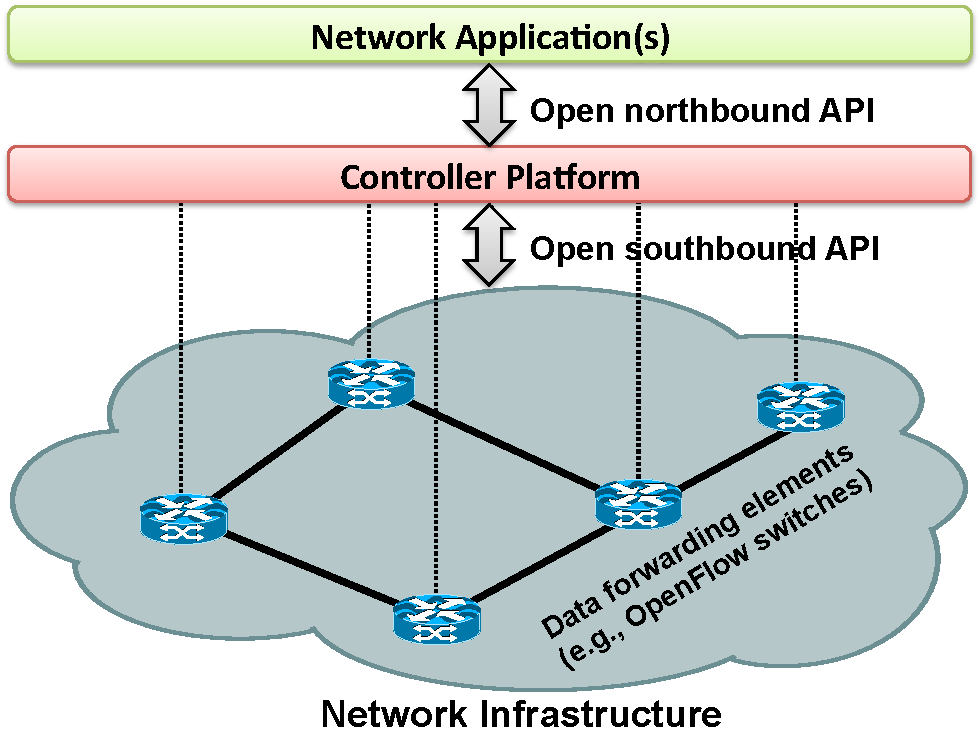
\includegraphics[width=0.95\columnwidth]{figures/fig1_sdn_simple.pdf}
\caption{Simplified view of an SDN architecture.}
\label{fig:sdn_simple}
\end{figure}

% Openflow as enabler
The separation of the control plane and the data plane can be realized
by means of a well-defined programming interface between the switches
and the SDN controller.  The controller exercises direct control over
the state in the data-plane elements via this well-defined application programming interface (API), as
depicted in Figure~\ref{fig:sdn_simple}.  The most notable example of
such an API is OpenFlow~\cite{mckeown2008, onf2013-3}.  An OpenFlow
switch has one or more tables of packet-handling rules (flow table).  
Each rule matches a subset of the traffic and performs certain actions (dropping,
forwarding, modifying, etc.) on the traffic.
%, matching the rule, which matches the rule.
Depending on the rules installed by a controller application, an
OpenFlow switch can -- instructed by the controller -- behave like a
router, switch, firewall, or perform other roles (e.g., load balancer, traffic shaper, and in general those of a
middlebox).

% SDN allows new abstractions and network evolution
An important consequence of the software-defined networking principles
is the \textit{separation of concerns} introduced between the
\textit{definition} of network policies, their \textit{implementation}
in switching hardware, and the \textit{forwarding} of traffic. This separation is key to the
desired flexibility, breaking the network control problem into
tractable pieces, and making it easier to create and introduce new
abstractions in networking, simplifying network management and
facilitating network evolution and innovation.

%SDN - current status
Although SDN and OpenFlow started as academic
experiments~\cite{mckeown2008}, they gained significant traction in the
industry over the past few years.  Most vendors of commercial switches
now include support of the OpenFlow API in their equipment. The SDN momentum 
was strong enough to make Google, Facebook, Yahoo, Microsoft, Verizon, and Deutsche Telekom fund Open Networking Foundation~(ONF)~\cite{onf2013-3} with the main
goal of promotion and adoption of SDN through open standards development driven by the users (i.e., equipment buyers) rather than the vendors (i.e., equipment manufacturers). 
  As the initial concerns with SDN scalability were addressed~\cite{yeganeh2013}
-- in particular the myth that logical centralization implied a
physically centralized controller, an issue we will return to later on
-- SDN ideas have matured and evolved from an academic exercise to
a commercial success. Google, for example, has deployed a software-defined
network to interconnect its data centers across the globe. This production 
network has been in deployment for 3 years, helping the company to improve 
operational efficiency and significantly reduce costs~\cite{jain2013-1}.
VMware's network virtualization platform, NSX~\cite{vmware2013},
is another example.  NSX is a commercial solution that delivers a
fully functional network in software, provisioned independent of the
underlying networking devices, entirely based around SDN principles.  As
a final example, the world's largest IT companies (from carriers and
equipment manufacturers to cloud providers and financial-services
companies) have recently joined SDN consortia such as the ONF  and the OpenDaylight initiative~\cite{opendaylight2013}, 
another indication of the importance of SDN from an industrial perspective.

%This paper
In this paper, we present a comprehensive literature survey on SDN organized as depicted in Figure~\ref{fig:conclusion}.  We start, in the next two sections, by explaining the context,
introducing the motivation for SDN and explaining the main concepts
of this new paradigm and how it differs from traditional networking.
Our aim in the early part of the survey is also to explain that SDN 
is not as novel as a technological advance.  Indeed, its existence 
is rooted at the intersection of a series of ``old'' ideas, 
technology drivers, and current and future needs. The concepts underlying SDN -- the 
separation of the control and data planes, the  flow abstraction upon
which forwarding decisions are made, the (logical) centralization of
network control, and the ability 
to program the network -- are not novel by themselves~\cite{feamster2013-2}.
However, the integration of already tested concepts with recent trends 
in networking -- namely the availability of merchant switch silicon and
the huge interest in feasible forms of network virtualization -- are
leading to this paradigm shift in networking.

Section~\ref{sec:layeredapproach} comes next and is the core of this
survey, presenting an extensive and comprehensive
analysis of the building blocks of an SDN infrastructure using a
bottom-up, layered approach.  The option for a layered approach is
grounded on the fact that SDN allows thinking of networking along two
fundamental concepts, which are common in other disciplines of 
computer science: a) separation of concerns (leveraging the concept of abstraction) and b) recursion.
Our layered, bottom-up approach divides the networking problem into eight parts: 1) hardware infrastructure, 2) southbound interfaces, 3) network virtualization (hypervisor layer between 
the forwarding devices and the network operating systems), 4) network operating 
systems (SDN controllers and control platforms), 5) northbound interfaces 
(to offer a common programming abstraction to the upper layers, mainly the network applications), 6) virtualization using slicing techniques provided by special purpose 
libraries and/or programming languages and compilers, 7) network 
programming languages, and finally 8) management applications. In addition, 
we also look at cross-layer problems such as debugging and troubleshooting 
mechanisms. The discussion in Section~\ref{sec:challenges} on ongoing research efforts, challenges, future work and opportunities concludes this paper.


\begin{figure*}[t]
\centering
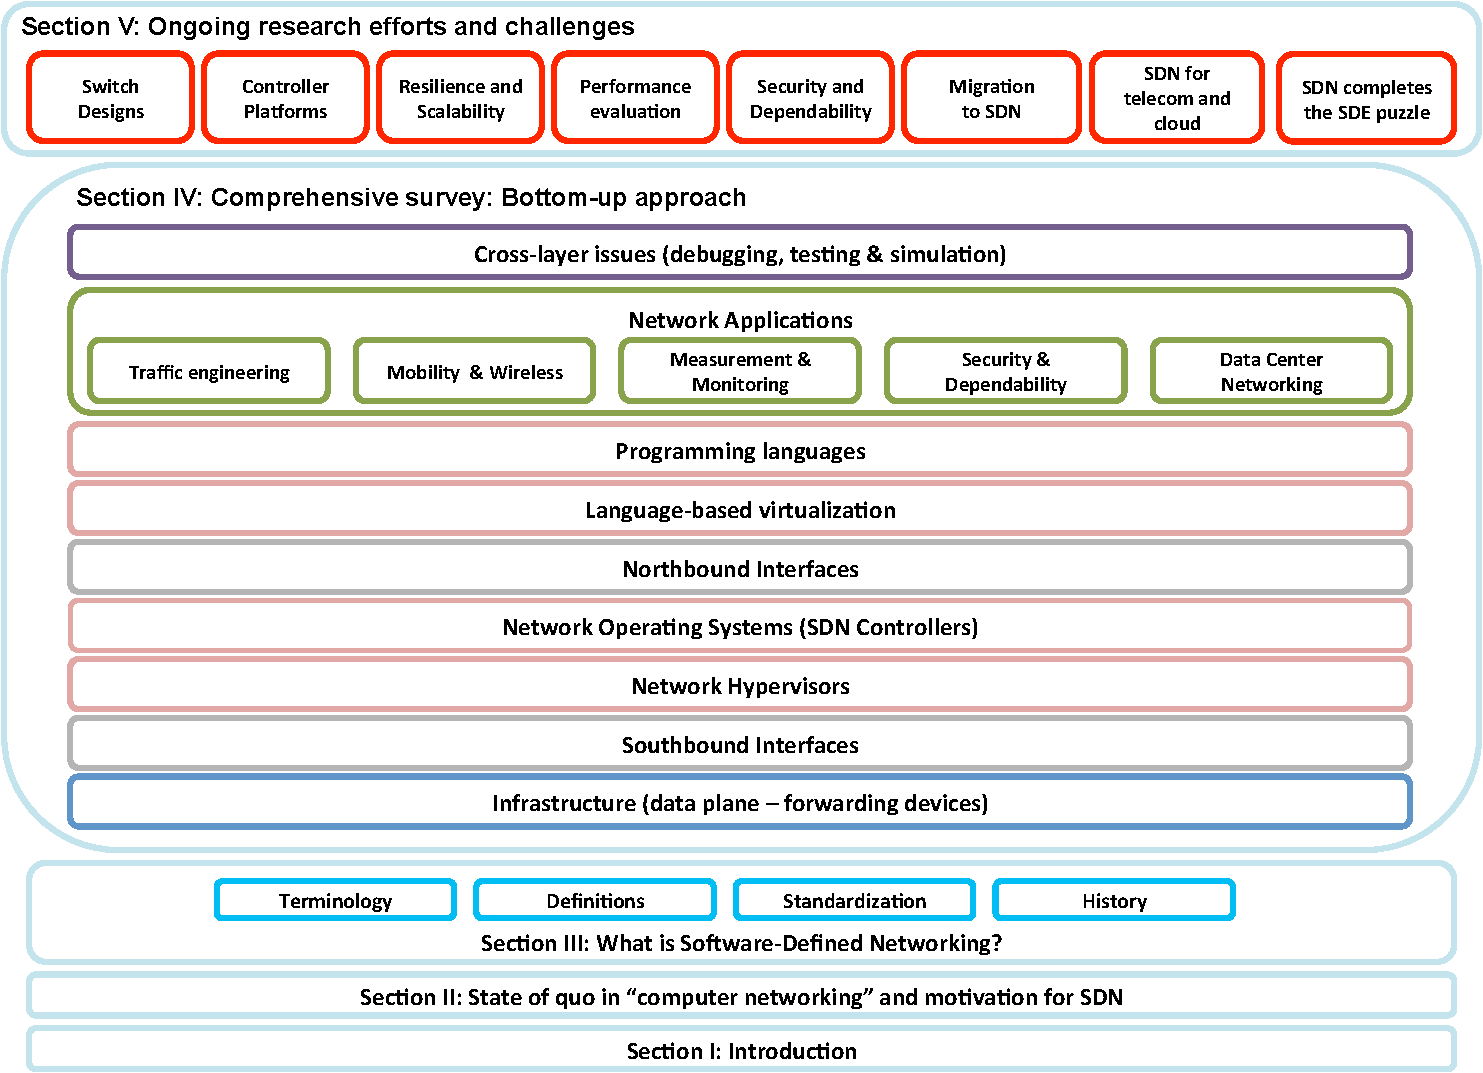
\includegraphics[width=0.95\textwidth]{figures/fig12_survey_condensed_overview.pdf}
\caption{Condensed overview of this survey on SDN.}
\label{fig:conclusion}
\end{figure*}

%(in short: scalability, security and dependability), several
%use cases and deployment scenarios, and finally we discuss open roads
%in SDN research, trying to foretell how this new paradigm will evolve.
%We pay particular attention to use case scenarios that are considered
%of crucial importance to network operators, such as optical and
%transport networks, datacenters, and wide area networks.
